\documentclass[conference,letterpaper]{IEEEtran}
\usepackage[T1]{fontenc}
\usepackage[utf8]{inputenc}
\usepackage{microtype,balance,amsmath,booktabs,tabularx,array,graphicx,tikz,enumitem}
\usepackage{pdflscape}
\usetikzlibrary{arrows.meta,positioning,shapes.geometric}
\usepackage[hidelinks,breaklinks]{hyperref}
\hypersetup{pdftitle={Parcel Guard: Owner-Managed Access and Persistent Incident Recovery in Webots},pdfauthor={Joshua Guico, Joe Jimenez, Brandon Lopez},pdfsubject={CS 5650 Project Progress Report 2}}
\urlstyle{same}
\setlength{\emergencystretch}{2em}
\setlist{nosep,leftmargin=*}
\setcounter{tocdepth}{2}
\renewcommand{\arraystretch}{1.15}
\pagestyle{plain}
\widowpenalty=10000\clubpenalty=10000
\newcolumntype{Y}{>{\raggedright\arraybackslash}X}
\newcommand{\code}[1]{\texttt{\small #1}}
\newcommand{\SecurityTests}{29}
\newcommand{\DashboardChecks}{33}
\newcommand{\SecurityGroups}{10}
\newcommand{\SecurityAssertions}{28}
\newcommand{\RecoveryTests}{26}
\newcommand{\Presence}{50/50}
\newcommand{\MacroF}{1.00}
\newcommand{\FalseAlarms}{0}
\newcommand{\Cycles}{100}
\newcommand{\Recovered}{100}
\newcommand{\Unauthorized}{0}
\newcommand{\SourceCount}{46}
\newcommand{\ReportCount}{13}

\begin{document}
\onecolumn\thispagestyle{empty}
\vspace*{0.85in}
\begin{center}
{\fontsize{20}{24}\selectfont\bfseries Package Delivery Security Box\par}
\vspace{0.18in}
{\fontsize{16}{20}\selectfont Webots Simulation for Secure Package Delivery\par}
\vspace{0.55in}
{\fontsize{14}{18}\selectfont CS 5650 Group Project: Progress Report 2\par}
\vspace{0.12in}
{\fontsize{14}{17}\selectfont Master of Science in Computer Science\par Department of Computer Science\par California State University, Los Angeles\par}
\vspace{0.5in}
{\fontsize{12}{15}\selectfont
\begin{tabular}{@{}ll@{}}
\textbf{Team Members:} & Joshua Guico\\ & Joe Jimenez\\ & Brandon Lopez\\[0.18in]
\textbf{Instructor:} & Dr. Jung Soo Lim\\\textbf{Semester:} & Fall 2026
\end{tabular}\par}
\vfill{\large November 17, 2026\par}
\end{center}\clearpage
\thispagestyle{empty}\tableofcontents\clearpage
\twocolumn
\title{Parcel Guard: Owner-Managed Access and Persistent Incident Recovery in Webots}
\author{Joshua Guico, Joe Jimenez, and Brandon Lopez\\M.S. Computer Science\\Department of Computer Science\\California State University, Los Angeles\\Fall 2026}
\maketitle
\begin{abstract}
Parcel Guard models a delivery security box in Webots. This second progress report extends the earlier fixed-code workflow with password-authenticated owner management, revocable one-use access codes, and persistent incident lockdown. An owner can authorize delivery or collection, revoke unused credentials, and run another delivery without resetting policy state. Unexplained activity revokes outstanding codes and ends owner sessions. Recovery requires a new owner sign-in and measured door closure and bolt locking. Local checkpoints retain pending events, credential state, cooldown and incidents across controller restarts. The current evaluation passes \SecurityTests{} security-policy tests, \DashboardChecks{} dashboard checks, and \SecurityGroups{} Webots security groups containing \SecurityAssertions{} assertions. Separate legacy-fixture benchmarks retain 50/50 package-presence decisions and macro F1 of 1.00 on generated scenarios. The report distinguishes these two evidence sets, describes implementation and failure behavior, and reports the follow-up test in which one tamper alert survived a lost acknowledgment and both controller restarts.
\end{abstract}
\begin{IEEEkeywords}Webots, access control, package delivery, incident response, persistent state, simulation.\end{IEEEkeywords}

\section{Introduction and Progress Since Report 1}
\subsection{Problem and Scope}
A delivery box must do more than accept a code. It must establish who may use that code, whether the parcel remains inside, whether the door and bolt actually reached secure positions, and what happens when access or device behavior is unexpected. Parcel Guard evaluates those conditions in a repeatable local simulation.

The original proposal limits the project to one box, one parcel at a time, and a Webots implementation \cite{proposal}. The first progress presentation and report established delivery and retrieval, role-separated temporary codes, sensed closure and locking, event classification, fault reporting, and simulated offline queuing \cite{progressone}. That baseline already passed its generated acceptance scenarios. Its visible workflow still used fixed demonstration PINs and a policy reset to issue another pair of credentials. Its queued state also depended on the running process.

This iteration changes the owner workflow. The default interactive world requires owner password sign-in for code management. The owner creates an eight-digit code for courier delivery or owner collection, chooses its lifetime, and can revoke it. Each successful code works once. A new code enables another delivery in the same policy session. Tamper events now cause an administrative lockdown, rather than only adding an event to the history.

The physical scope remains unchanged. The model does not establish forced-entry resistance, weather protection, safe human interaction, carrier identity or real notification delivery. The ordinary box controller reads Webots devices; separate Supervisor fixtures create stimuli and assign evaluation truth. The report describes a local course prototype, not a deployed security product.

\subsection{Implemented Changes}
Report 1 identified restart recovery and sensor faults as follow-up work. Table~\ref{tab:changes} shows what was implemented and verified by Report 2. The two milestones use the same Webots model and measured locking rule. The new owner console changes how access is issued, repeated and withdrawn.
\begin{table*}[t]\centering\small
\caption{Implemented progress since the first report.}\label{tab:changes}
\begin{tabularx}{\textwidth}{@{}p{.17\textwidth}YY@{}}\toprule
Area & Report 1 (October) & Report 2 (November)\\\midrule
Owner control & Fixed role-specific demonstration PINs. & Password sign-in lets the owner issue and revoke expiring, one-use delivery or collection codes.\\
Repeated deliveries & Reset policy to reissue demo PINs. & A second delivery was verified in the same policy session with a fresh code.\\
Tamper response & Record suspected tampering in the event log. & Revoke outstanding codes, end owner sessions and keep lockdown active until a fresh owner sign-in and measured locking.\\
Restart recovery & Queue and credential-use state held in memory. & Local checkpoint restores pending alerts and security state. Ten queued alerts survived a Webots controller restart.\\
Fault coverage & Non-finite feedback and motion timeouts. & Added tests for out-of-range feedback, frozen bolt readings and strong impacts during approved access.\\\bottomrule
\end{tabularx}\end{table*}

\subsection{Team Responsibilities}
The proposal assigns Joshua Guico project planning, integration, presentation and report coordination; Joe Jimenez the enclosure, sensors and simulation scenarios; and Brandon Lopez controller, interface and automated testing responsibilities \cite{proposal}. These are the original responsibility allocations, not a new measurement of individual effort. Integration, evidence review and presentation preparation remain shared activities.

\section{System Architecture}
\subsection{Device and Policy Separation}
Webots supplies the simulated devices and physics environment \cite{webots}. Twenty-five downward distance rays form a $5\times5$ parcel array. Door and bolt position feedback, plus a door accelerometer, enter a shared filter every 32~ms. The filter validates values, applies distance hysteresis, and requires three consistent samples before changing parcel state. The adapter publishes status every third step, or 96~ms.

Figure~\ref{fig:architecture} shows the current data flow. The Python policy owns access decisions, event rules and actuator targets. A security component handles owner sessions and credentials; a local store checkpoints the durable policy state. Motor commands and measured feedback remain distinct. A target command alone never proves closure or locking.
\begin{figure*}[t]\centering
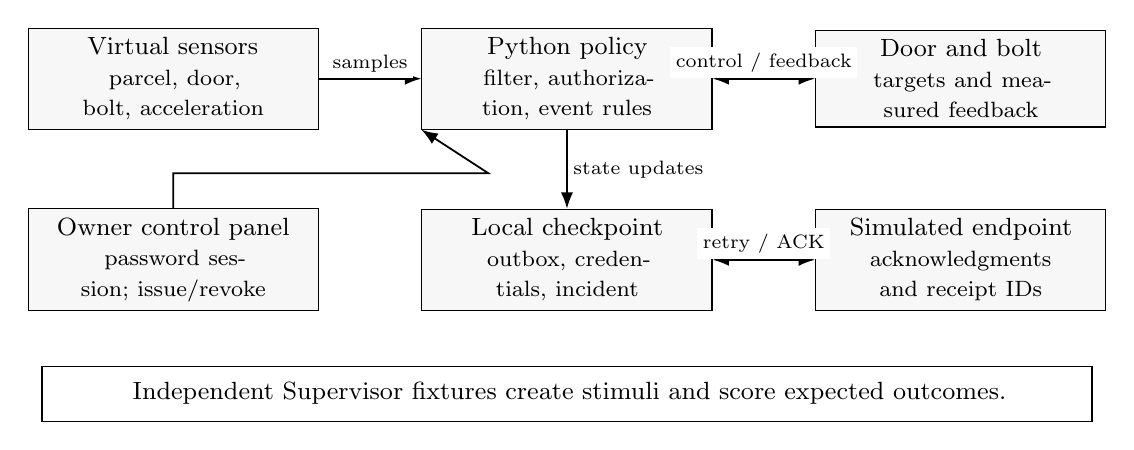
\begin{tikzpicture}[x=1cm,y=1cm,>=Latex,font=\small,
box/.style={draw,align=center,text width=3.45cm,minimum height=1.05cm,fill=black!3},
arr/.style={->,line width=.65pt},lab/.style={font=\scriptsize,fill=white,inner sep=2pt}]
\node[box] (sensors) at (0,0) {Virtual sensors\\\footnotesize parcel, door, bolt, acceleration};
\node[box] (policy) at (5,0) {Python policy\\\footnotesize filter, authorization, event rules};
\node[box] (motors) at (10,0) {Door and bolt\\\footnotesize targets and measured feedback};
\node[box] (owner) at (0,-2.3) {Owner control panel\\\footnotesize password session; issue/revoke};
\node[box] (store) at (5,-2.3) {Local checkpoint\\\footnotesize outbox, credentials, incident};
\node[box] (endpoint) at (10,-2.3) {Simulated endpoint\\\footnotesize acknowledgments and receipt IDs};
\draw[arr] (sensors)--node[lab,above]{samples}(policy);
\draw[<->,line width=.65pt] (policy)--node[lab,above]{control / feedback}(motors);
\draw[arr] (owner.north)--(0,-1.2)--(4,-1.2)--(policy.south west);
\draw[arr] (policy)--node[lab,right]{state updates}(store);
\draw[<->,line width=.65pt] (store)--node[lab,above]{retry / ACK}(endpoint);
\node[draw,align=center,text width=13.1cm,minimum height=.7cm] at (5,-4.0) {Independent Supervisor fixtures create stimuli and score expected outcomes.};
\end{tikzpicture}
\caption{Current architecture. The ordinary Robot uses device feedback; test fixtures alone can inspect or manipulate scene truth. The simulated endpoint is separate from the sender checkpoint.}\label{fig:architecture}
\end{figure*}

\subsection{Physical Security and Administrative State}
Physical secured status is derived from valid feedback $V$, closed door $D_c$, locked bolt $B_l$, fault $F$, active grant $G$, and closing operation $C$:
\begin{equation}S=V\land D_c\land B_l\land\neg F\land\neg G\land\neg C.\end{equation}
Administrative lockdown $L$ is separate. A physically secured box can still reject all new access because $L$ remains active. The interface therefore shows door, bolt and parcel feedback alongside the lockdown banner. Faults remain visible during an incident, and clearing the incident requires $S$ to hold.

Normal actuator sequencing is unchanged: retract the bolt, confirm retraction, open the door, permit authorized handling, close the door, confirm closure, extend the bolt and confirm locking. An access grant ends on close, deadline, sensor failure or an incident. The runtime holds bolt retraction when valid closed-door feedback is unavailable.

\section{Owner Management and Credential Design}
Figure~\ref{fig:workflow} traces owner code management, access decisions, delivery confirmation and lockdown recovery.
\subsection{Password-Authenticated Management Sessions}
The owner signs in using a password. The implementation stores a PBKDF2-HMAC-SHA256 verifier with a random salt and 200,000 iterations. Python provides the PBKDF2 primitive through \code{hashlib} \cite{pythonhash}. This implementation choice is a concrete local control, not a claim that the surrounding application has production-grade authentication.

A successful sign-in creates a random bearer session valid for 300 simulated seconds. A new successful sign-in immediately replaces the previous session. Sign-out, controller restart and tampering invalidate the session. Sessions are not restored from disk and do not appear in shared status or audit exports. Five wrong owner passwords pause management sign-in for 60 simulated seconds; the failure counter and pause survive restart.

Owner authentication does not itself unlock the door. It authorizes management actions: issue a delivery or collection code, revoke a selected credential, or clear an incident after measured security returns. A courier code cannot perform those management actions. A separate password for management keeps the door-entry surface distinct from the owner console.

\subsection{Temporary Access Codes}
Each issued credential contains an ID, purpose, keyed code digest, expiry, used flag and revoked flag. Codes contain eight decimal digits generated using Python's cryptographic random source. The owner selects a lifetime between 30 and 3600 simulated seconds. Plaintext is returned once to the requesting owner interface, while public status exposes only metadata.

A credential can grant access only if it matches the entered value, is not revoked, has not been consumed, has not expired, matches the requested role and is otherwise compatible with device state. Courier access is denied when a parcel is already present. Concurrent access and replayed door-entry request IDs remain denied. A role mismatch does not consume a valid credential.

Successful use marks the credential consumed before the grant can drive opening. The policy checkpoints the change. If saving fails, the command does not return a successful access result and the controller enters a storage fault. This ordering avoids opening first and recording one-use state afterward.

Revocation is terminal for that credential. Clearing a later lockdown does not reactivate it. A new credential ID and code are required. The demonstration retains a bounded history of 128 issued credentials; this bound keeps the local course prototype small and is not an operational retention policy.

\subsection{Delivery and Retrieval Rules}
A debounced empty-to-present parcel transition during approved open-door courier access marks a delivery pending. The controller records completed delivery only after the parcel remains present, the door closes and the bolt reaches locked feedback without an active grant or fault. A blocked bolt therefore cannot produce a successful delivery confirmation.

A present-to-empty transition during owner collection access records retrieval. Unapproved parcel changes, unexpected door opening and unapproved impacts produce tamper events. Normal authorized movement retains its context. This design remains a deterministic rule system, not a learned classifier or an identity-recognition system.

\section{Incident Response and Restart Recovery}
\subsection{Persistent Lockdown}
In security mode, a tamper event revokes every issued access code, invalidates all owner sessions, cancels any active grant and records the incident. The control panel changes to \code{LOCKDOWN}. Device control still attempts closure and measured locking; administrative policy never bypasses an unresolved sensor or actuator fault.

The owner must sign in again with the password to clear the incident. Clearance is denied unless measured physical security holds. The old owner session cannot clear lockdown, and previously issued codes remain revoked afterward. The \code{reset\_logic} fixture command is rejected in security mode, preventing the visible New session control from erasing incidents or reissuing door credentials.

The simulated attack sequence exercises an ordinary unapproved impact while the box is secured. A separate stronger-impact threshold above $35\,\mathrm{m/s^2}$ remains active during authorized handling and post-close settling. A usable accelerometer can report that event even when another sensor is invalid. These fixed thresholds require calibration before a physical design could rely on them.

\subsection{Atomic Local Checkpoints}
The interactive controller writes a local JSON checkpoint containing event namespace and next ID, pending and acknowledged records, credential state, door-entry replay IDs, failure history, cooldown, link state and incident. The separate runtime JSONL file remains an audit export; it is not the recovery database.

Saving writes a temporary file, flushes and synchronizes its data, atomically replaces the previous checkpoint, and synchronizes the containing directory. A checksum detects accidental damage. It is not a signature or protection against a malicious host. The state contains private digest-key material and a password verifier, and is not encrypted.

On restart, the controller retains original pending event IDs and the incident, but cancels access and discards owner sessions. Fresh stable feedback is required before secured status. An incomplete pending delivery is cancelled because uninterrupted parcel custody cannot be inferred from the checkpoint alone. If the world epoch changes or simulated time moves backward, issued credentials are revoked rather than gaining a fresh lifetime.

Existing security checkpoints upgrade to the password-only schema without discarding the password verifier, issued code digests, queue or incident. The migration retains the digest-key bytes while removing obsolete fields. This path has its own regression test.

\subsection{Sensor and Actuator Faults}
The filter rejects non-finite readings and values outside the modeled ranges: distance 0 to 0.65~m, door angle $-0.06$ to 1.50~rad, and bolt travel $-0.02$ to 0.10~m. These ranges include margin around modeled travel and sensor noise. Invalid readings reset consecutive-sample counts, deny access and prevent secured status until three stable valid samples return.

Frozen bolt feedback during commanded motion fails the existing two-second target timeout. Recovery requires measured target feedback after the fixture releases the fault. These checks do not reliably diagnose a plausible frozen parcel array or a joint reading frozen at an already-commanded target. The report keeps those unresolved cases separate from passing fault trials.

\section{Evaluation Method}
\subsection{Separate Evidence Sets}
The evaluation runs two complementary paths. Original acceptance worlds retain legacy fixture credentials to preserve a comparable package-detection, event-classification, motion and offline-recovery benchmark. The dedicated \code{delivery\_box\_security.wbt} uses the default owner-managed policy and independently measured device feedback.

Consequently, the original macro F1 is not presented as the classification score of every managed-code scenario. The current security suite instead verifies the complete workflow, including a delivery and collection, a second delivery in the same policy session, revocation, exact expiry, an incident, real controller restart and owner recovery.

\subsection{Policy, Interface and Simulation Checks}
The \code{security\_layers.py} suite checks password-only login, malformed passwords, sign-in throttling, immediate repeat sign-in, session invalidation, role scope, expiry, one-use consumption, revocation, migration and injected write failures. Tests use temporary stores. The previous recovery suite additionally includes an abrupt child-process exit and atomic-replacement failures.

The dashboard suite exercises the actual page script with recorded status and injected fault states. It verifies password-only form submission, cleared owner inputs, authenticated code controls, and lockdown clearance that waits for physical security. Chromium layout checks render protected, incident and recovered snapshots at desktop and 390-pixel widths. These interface checks are not physical-security trials.

The independent Webots runner receives private command replies on a separate test channel, uses actual door/bolt and parcel feedback, and exports assertions without plaintext codes or bearer tokens. The fixture password is isolated from the interactive owner's saved state. Full-run source and report hashes bind the evidence to the evaluated implementation \cite{evidence}.

\section{Results and Discussion}
\subsection{Current Owner-Managed Workflow}
All \SecurityTests{} new security-policy tests, \DashboardChecks{} dashboard checks, and \SecurityGroups{} Webots security scenario groups pass. The simulation groups contain \SecurityAssertions{} assertions. Table~\ref{tab:securityresults} summarizes outcomes; saved JSON retains the individual assertions.
\begin{table*}[t]\centering\small
\caption{Current security workflow results from the dedicated Webots suite.}\label{tab:securityresults}
\begin{tabularx}{\textwidth}{@{}p{.24\textwidth}Y@{}}\toprule
Scenario & Observed outcome\\\midrule
Secure default and sign-in & Fixed fixture PINs denied; wrong/missing password denied; password-only and immediate repeat sign-in accepted.\\
Code management & Owner revocation accepted; revoked and expired credentials could not grant access.\\
Managed parcel workflow & Delivery completed after measured locking; owner collection completed; a second delivery used the same policy session.\\
Incident response & Outstanding credentials revoked; old owner session invalidated; a previously valid code could not open the box.\\
Restart and recovery & Reset could not bypass lockdown; incident and revocations survived controller restart; password sign-in and secure clearance restored service.\\
Private-data redaction & Owner password, newly issued codes and bearer sessions absent from shared status.\\\bottomrule
\end{tabularx}\end{table*}

A restart or incident requires a new password-authenticated owner session before clearance. The previous session cannot authorize recovery. These session checks complement one-use credentials, expiry, revocation and password throttling; successful owner sign-in still cannot override invalid physical feedback.

\subsection{Benchmark Comparison and New Recovery Coverage}
Report 1 already met the proposal targets. Table~\ref{tab:baseline} compares its October results with the November rerun of the same fixture-code benchmark \cite{progressone,evidence}. The benchmark scores held steady. The new evidence covers owner-managed access, persistent lockdown and controller restart recovery.
\begin{table}[t]\centering\small
\caption{October baseline and November rerun with fixture PINs.}\label{tab:baseline}
\begin{tabular}{@{}lrr@{}}\toprule
Measure & Report 1 & Report 2\\\midrule
Package presence & 50/50 & \Presence{}\\
Four-class macro F1 & 1.00 & \MacroF{}\\
Non-tamper false alarms & 0/45 & \FalseAlarms{}/45\\
Completed motor cycles & 100/100 & \Cycles{}/100\\
Unauthorized unlocks & 0/30 & \Unauthorized{}/30\\
Recovered offline events & 100/100 & \Recovered{}/100\\\bottomrule
\end{tabular}\end{table}

The \RecoveryTests{} recovery and fault tests added since Report 1 pass, along with all 38 original policy regressions. Seven additional Webots recovery groups provide evidence for ten queued impact events surviving a real controller restart, lost-ACK retries, safe restart during access, invalid sensor ranges, frozen bolt feedback and strong impact during access. This suite keeps the receiver running. A separate follow-up tests both sides restarting after a lost acknowledgment.

\subsection{Follow-Up: Durable Alert Receipts}
The receiver stores the alert in SQLite under its session and event ID before sending an acknowledgment (ACK). A retry receives an ACK for the existing record. In Webots, the receiver stored a tamper alert and its ACK was dropped. Both controllers restarted while the link was paused. The sender reloaded its pending alert and the receiver reloaded its receipt. After reconnection, the receiver recognized the retry, retained one stored alert, and sent the ACK that emptied the sender queue. The measured sequence is in \code{webots\_alert\_recovery.json}.

\subsection{Interface Evidence}
Figure~\ref{fig:lockdown} is a recorded status snapshot from the security evaluation. It shows a physically closed and locked enclosure that remains administratively blocked. The owner console provides password sign-in, purpose/lifetime selection, one-use code creation and revocation. The screenshot is evidence of the displayed state, not a separate successful authentication trial.
\begin{figure*}[t]\centering
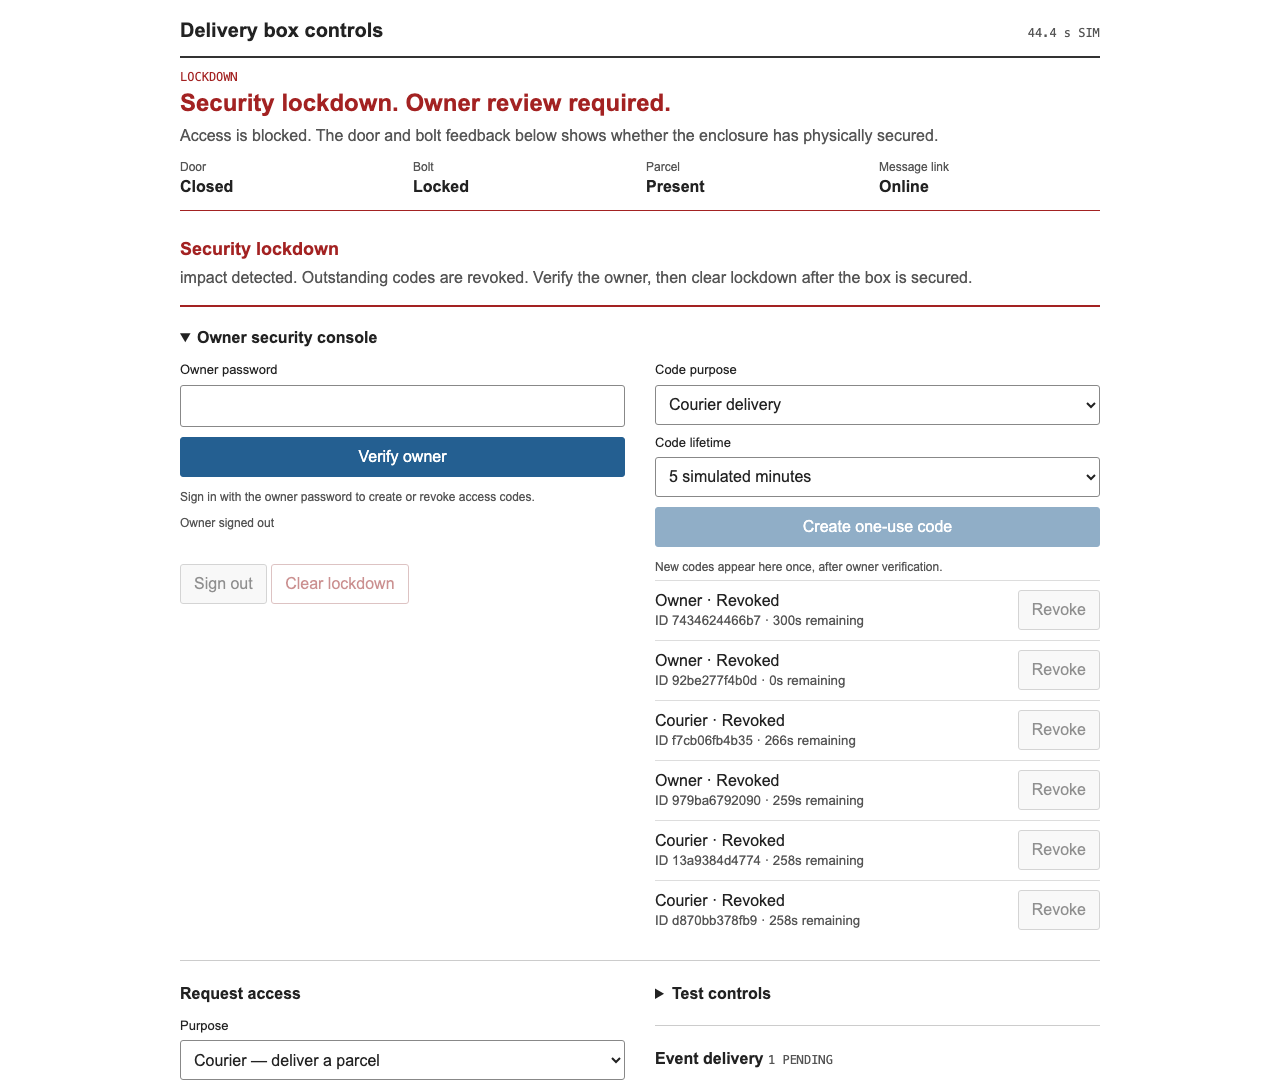
\includegraphics[width=.92\textwidth,trim=180 771 180 55,clip]{assets/lockdown.png}
\caption{Recorded Webots lockdown state. Physical door and bolt feedback remain visible while new access is blocked pending owner review. The full evaluation, rather than the screenshot alone, verifies revocation and recovery.}\label{fig:lockdown}
\end{figure*}

\subsection{Interpretation and Limits}
Perfect results on known generated scenario families should not be extrapolated to field behavior. Parcel movement is scripted, the physical model does not establish lock strength, and the interface exposes trusted fault fixtures. A local host can inspect or alter private state. A password verifier and keyed credential digest do not create an authenticated network boundary.

The sender checkpoint is tested across process/controller restart and injected storage errors, but physical power interruption is untested. The dual-restart test retained both local stores. It measures one record at the simulated receiver. Storage loss and external notification delivery are outside that test.

\section{Next Steps and Conclusion}
Receipt recovery during physical power interruption remains a follow-up test. Independent parcel sensing or explicit diagnostics are needed for plausible frozen readings. Hardware traces should guide impact calibration, and any physical prototype would require enclosure, safe-motion and forced-entry testing. A networked version would also need a separately authenticated operational interface and protected secret storage.

The current iteration provides a demonstrably different owner workflow: authorize access, revoke a credential, trigger persistent incident response, and restore service through password sign-in and measured security. It retains local delivery and retrieval, while keeping baseline classification results and new security-workflow evidence distinct.

\appendices
\section{Reproduction and Class Demonstration}
Use Webots R2025a, Python 3.10 or newer, and the existing demo-studio Node dependencies for dashboard checks. \code{python3 scripts/verify\_progress2.py} verifies saved evidence without starting Webots. \code{python3 scripts/run\_all.py} regenerates worlds and repeats the numerical benchmark, recovery tests, interface checks and separate owner-security scenario. The manifest records \SourceCount{} source/configuration hashes and \ReportCount{} passing report files; source remains fixed throughout that run.

For class, open \code{worlds/delivery\_box.wbt}, choose real-time speed and open its Robot Window. Sign in with the local demo owner password, create and revoke a courier code, complete an authorized delivery and collection, then inject ordinary Impact while the box is secured. Show that outstanding codes are revoked and the owner session ends. Restart the controller, sign in again and clear the incident only after measured security returns. Issue a new code to resume operation. The speaker guide includes a short live-demonstration sequence and a screenshot fallback.

\balance
\begin{thebibliography}{9}
\bibitem{proposal} J. Guico, J. Jimenez, and B. Lopez, \emph{Package Delivery Security Box: Webots Simulation for Secure Package Delivery}, CS 5650 project proposal, California State University, Los Angeles, Sept. 2026. Supplied project materials.
\bibitem{progressone} J. Guico, J. Jimenez, and B. Lopez, \emph{Package Delivery Security Box: Project Progress Report 1}, CS 5650, Oct. 18, 2026, Secs. IV--VII. Saved benchmark in \code{results/progress1\_baseline/REPORT.md}.
\bibitem{webots} Cyberbotics, \emph{Webots User Guide and Reference Manual}, R2025a. \url{https://cyberbotics.com/doc/guide/index?version=R2025a}.
\bibitem{pythonhash} Python Software Foundation, ``hashlib: Key derivation,'' Python documentation. \url{https://docs.python.org/3/library/hashlib.html#key-derivation}.
\bibitem{evidence} Parcel Guard project, ``Saved evaluation reports,'' Nov. 2026. The numerical, security, and restart reports are indexed in the evaluation manifest in the accompanying project package.
\end{thebibliography}
\clearpage
\onecolumn
\begin{landscape}
\section{Security Workflow}
\begin{figure}[h!]
\centering
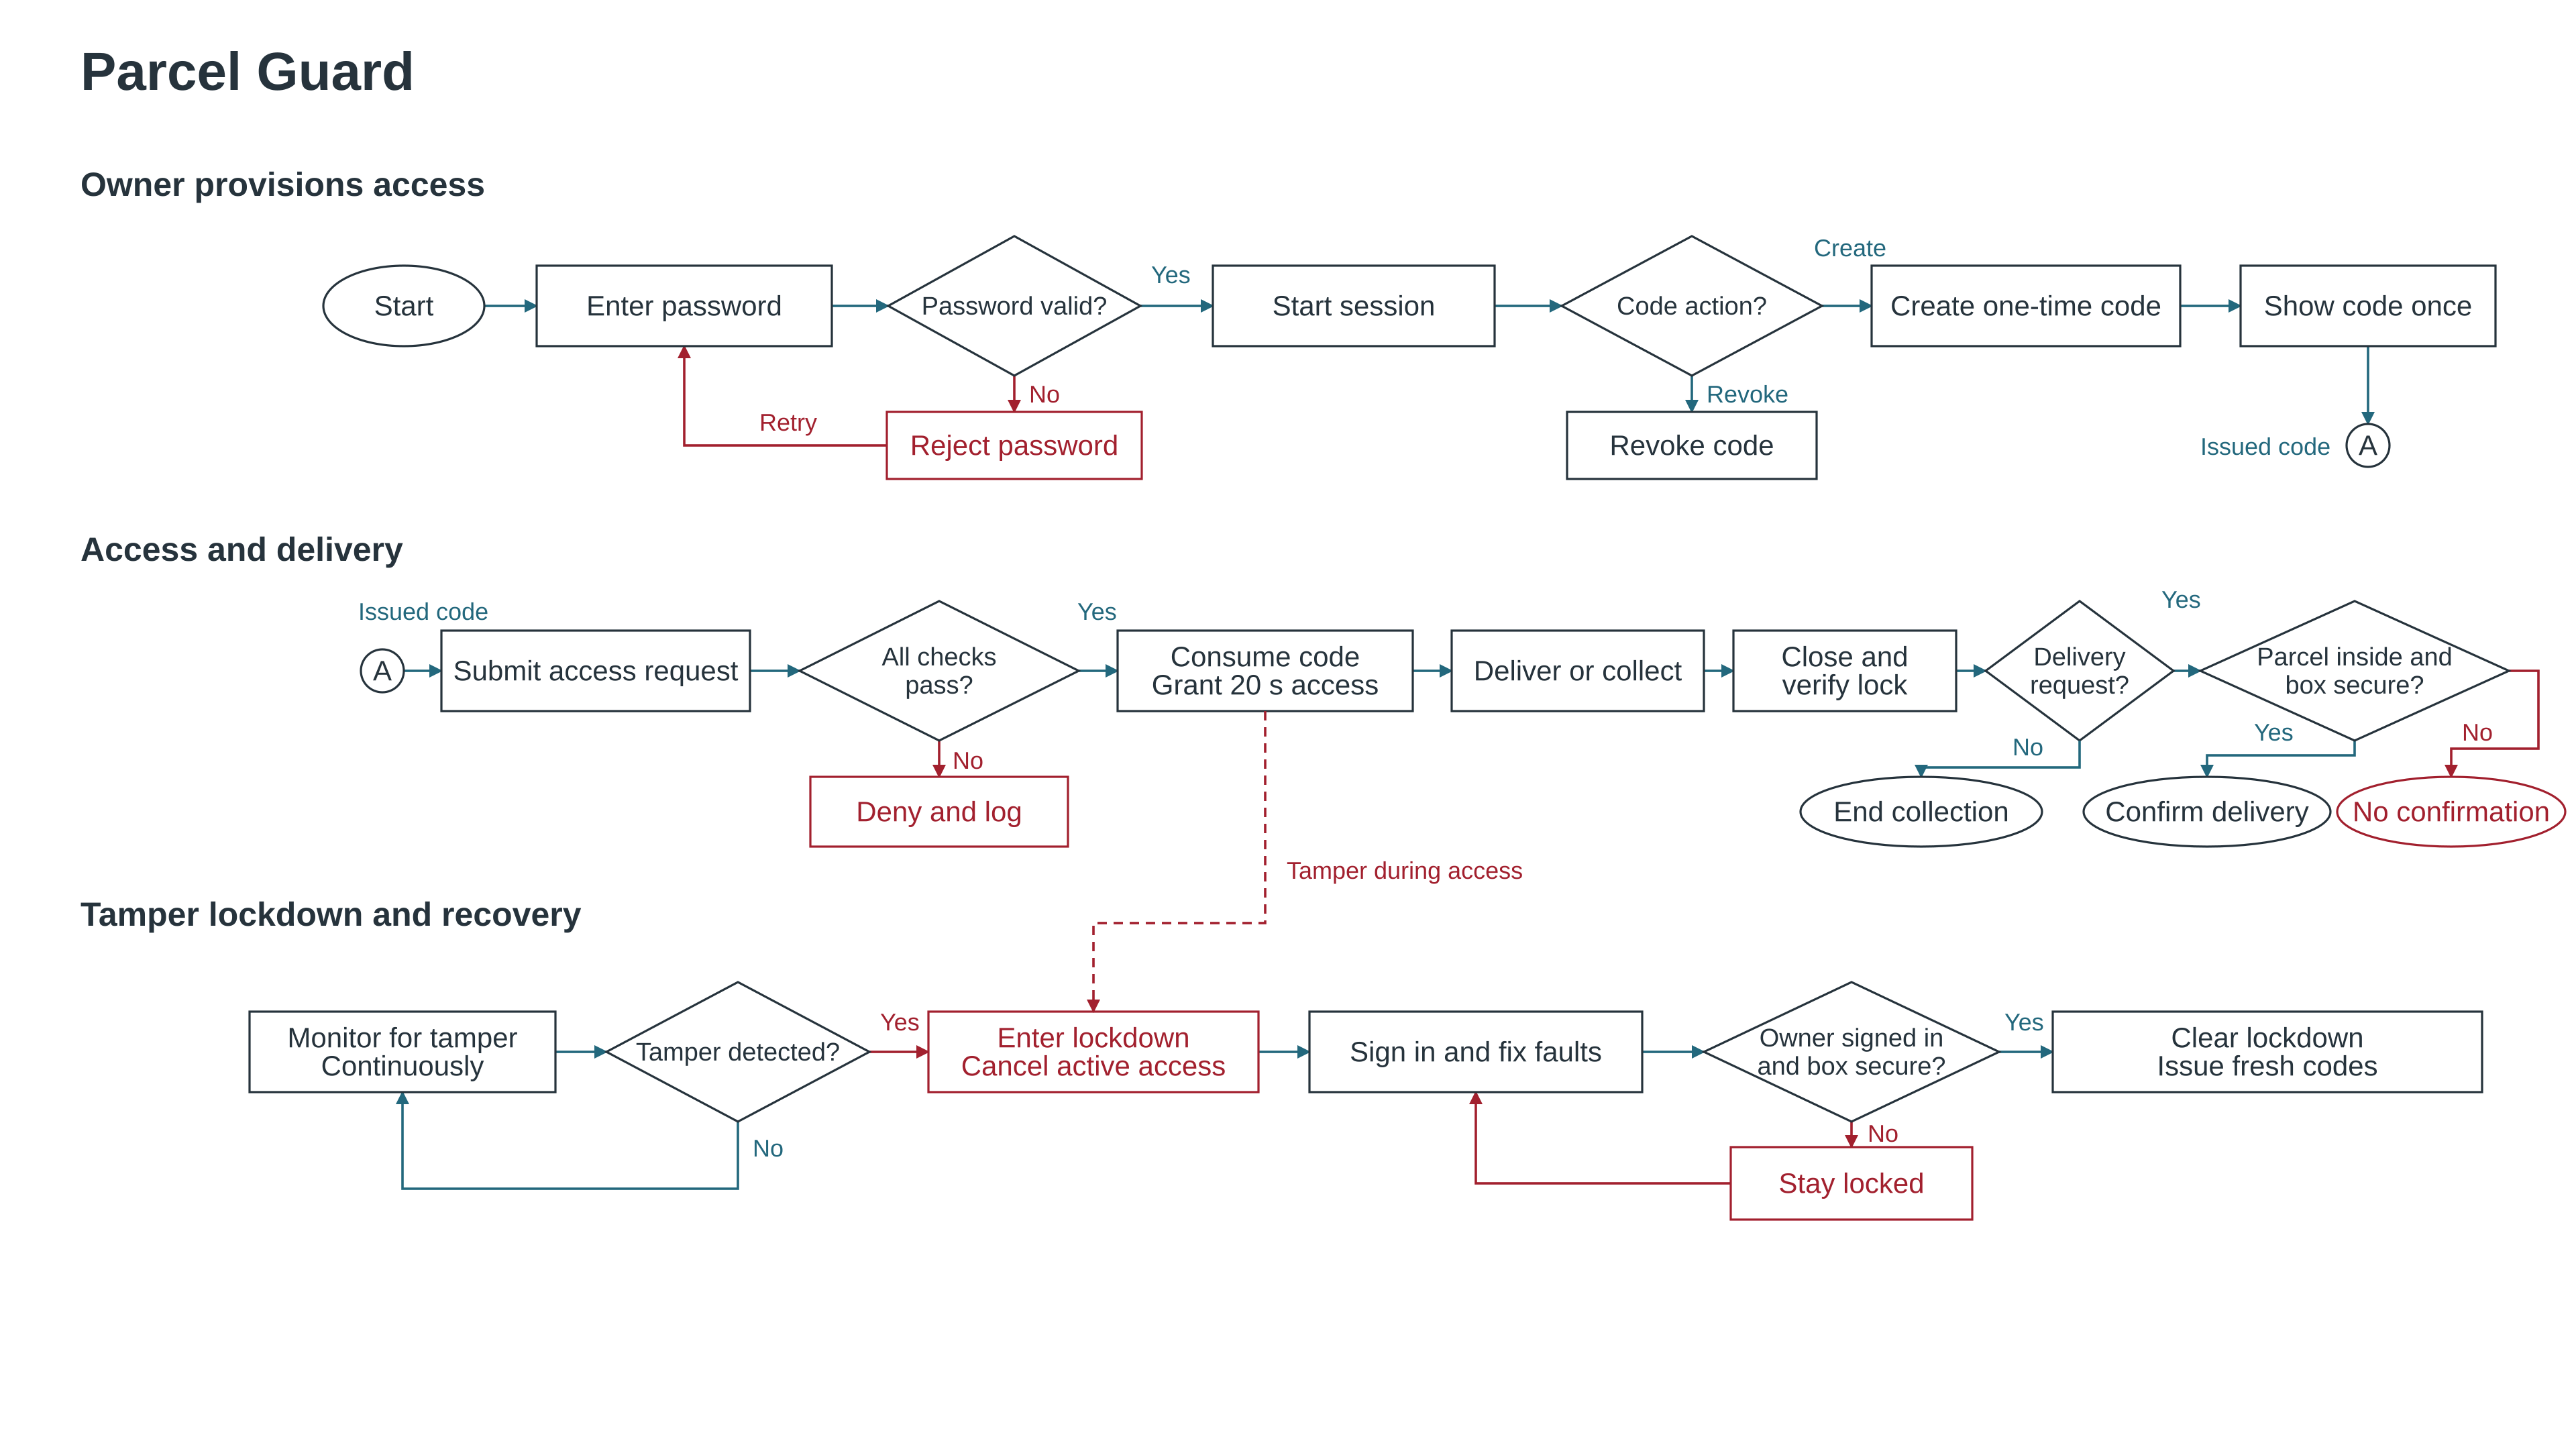
\includegraphics[width=\linewidth,trim=100 305 0 205,clip]{assets/parcel-guard-workflow.png}
\caption{Parcel Guard security workflow. Connector A carries the issued code to the access request. All times are simulated. Lockdown revokes issued codes, ends the owner session, and cancels active access. A failed recovery check keeps administrative lockdown active while the door and bolt are secured.}\label{fig:workflow}
\end{figure}
\end{landscape}
\end{document}
